\documentclass{article}
\usepackage[margin=1in]{geometry}
\usepackage{graphicx}
\graphicspath{{p5_phase_b_pilot/}{reports/p5_phase_b_pilot/}{p4_phase_b_pilot/G1/}{reports/p4_phase_b_pilot/G1/}}
\title{Flight Departure Delay Prediction}
\begin{document}
\maketitle
\section{Problem and checkpoints}
Owner: P1/P3. Pending reviewed contribution.
\section{Dataset and EDA}
Owner: P2. Pending reviewed contribution.
\section{Cleaning and UTC handling}
Owner: P1. Pending reviewed contribution.
\section{Split design and evaluation}
Owner: P1. Pending reviewed contribution.
\section{Column audit}
Owner: P2. Pending reviewed contribution.
\section{Feature engineering}
Owner: P3. Pending reviewed contribution.
\section{Classical models and PCA comparison}
The 20,000-flight paired development pilot compared schedule and calendar predictors (G0) with the addition of backward-looking origin congestion (G1). Each search used the four July--October folds and three common month-stratified training draws. We ranked configurations by mean average precision (PR-AUC), refit selected settings on all eligible training flights in each pilot fold, and scored the full validation portion of that fold. July and September pilot prevalence was 28.60\% and 16.05\%, respectively. Fold--seed spread includes this time variation.

We varied Decision Tree depth and minimum leaf size before tuning the cost-complexity penalty. Supplementary pruning values came from the first fold's training draw. Random Forest tuning varied depth, minimum leaf size, feature sampling, and tree count. G0 used identical schedule inputs at both horizons. Its selected tree used depth 12, a minimum leaf size of 200, and zero pruning penalty. Its forest used 128 trees and reached PR-AUC 0.379 and ROC-AUC 0.694 at both checkpoints.

Centered PCA was fitted inside each training pipeline after imputation, scaling the numeric block, and one-hot encoding. We compared 90\% and 95\% explained-variance targets with matching Random Forest and logistic controls. In G0, the selected 90\% PCA policy retained 50 components per full-fold fit. It changed mean PR-AUC by $-0.023$ for the matched forest and $+0.011$ for logistic regression. The representative loadings are expressed in each fitted encoded basis. The G1 matched forest pair uses a common 64-tree cap in both arms to bound the cost of fitting dense projections.

\begin{center}
\small
\begin{tabular}{lcccc}
 & \multicolumn{2}{c}{6 hours} & \multicolumn{2}{c}{1 hour} \\
G1 model & ROC-AUC & PR-AUC & ROC-AUC & PR-AUC \\ \hline
Majority & $0.500\pm0.000$ & $0.218\pm0.051$ & $0.500\pm0.000$ & $0.218\pm0.051$ \\
Decision Tree & $0.671\pm0.008$ & $0.352\pm0.054$ & $0.685\pm0.007$ & $0.382\pm0.057$ \\
Random Forest & $0.699\pm0.009$ & $0.394\pm0.062$ & $0.706\pm0.007$ & $0.424\pm0.064$ \\
Matched RF control & $0.698\pm0.010$ & $0.392\pm0.062$ & $0.703\pm0.008$ & $0.420\pm0.066$ \\
Matched RF with PCA & $0.689\pm0.006$ & $0.368\pm0.070$ & $0.700\pm0.007$ & $0.407\pm0.057$ \\
\end{tabular}
\end{center}

At 6h, the selected pruning penalty was about 0.000148. It removed about 116 leaves on average relative to the unpruned tree at the same depth and minimum leaf size and improved sampled-search PR-AUC from 0.339 to 0.342. The G1 forest selected 256 trees at both checkpoints with mean fit and scoring times of 3.39 and 2.73 seconds. The matched 90\% PCA fits retained 41 components and changed PR-AUC by $-0.024$ and $-0.013$ for the forest and by $+0.016$ and $+0.011$ for logistic regression at 6h and 1h. The October G1 fit had 279 encoded columns at 4.3\% density. Distance and scheduled duration had the largest first-component loadings.

Permutation importance for the selected G1 tree ranked scheduled UTC hour cosine first at 6h and the recent origin late-departure rate first at 1h. The representative October 1h tree used a root threshold of 0.2235 on recent origin late rate. Its two training child nodes had late rates of 15.9\% and 38.9\%. The full G0--G2 validation and test tables require the frozen feature release and team run.

\begin{figure}[htbp]\centering
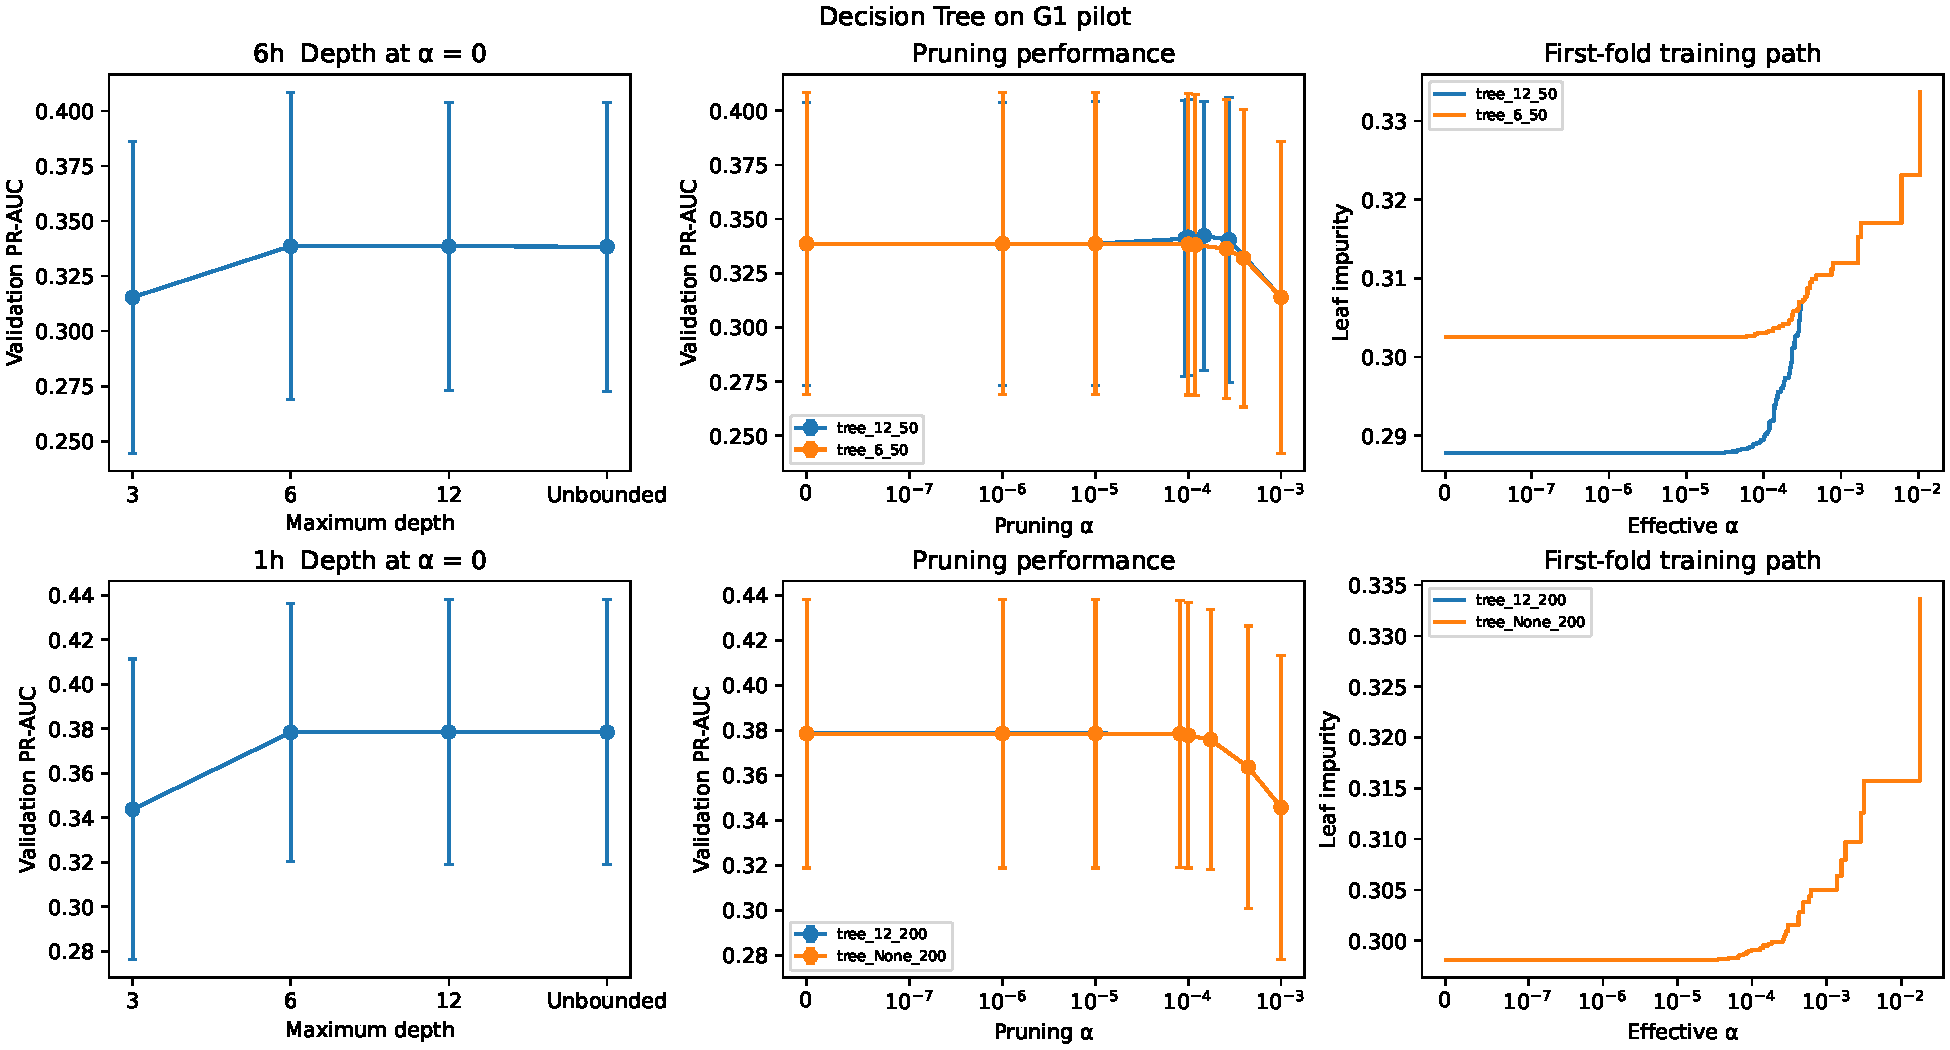
\includegraphics[width=\linewidth]{decision_tree.pdf}
\caption{G1 pilot Decision Tree depth and pruning comparisons.}
\end{figure}
\begin{figure}[htbp]\centering
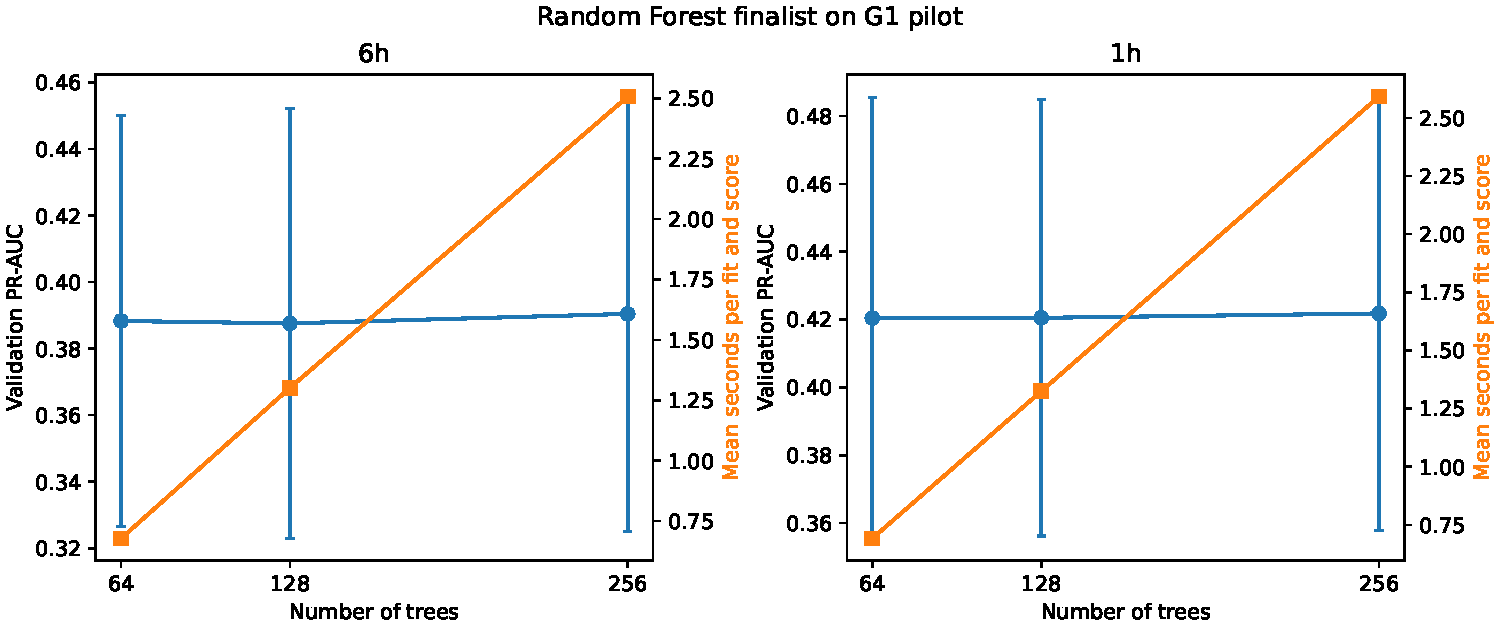
\includegraphics[width=\linewidth]{random_forest.pdf}
\caption{G1 pilot Random Forest finalist scores and runtime as tree count varies.}
\end{figure}
\begin{figure}[htbp]\centering
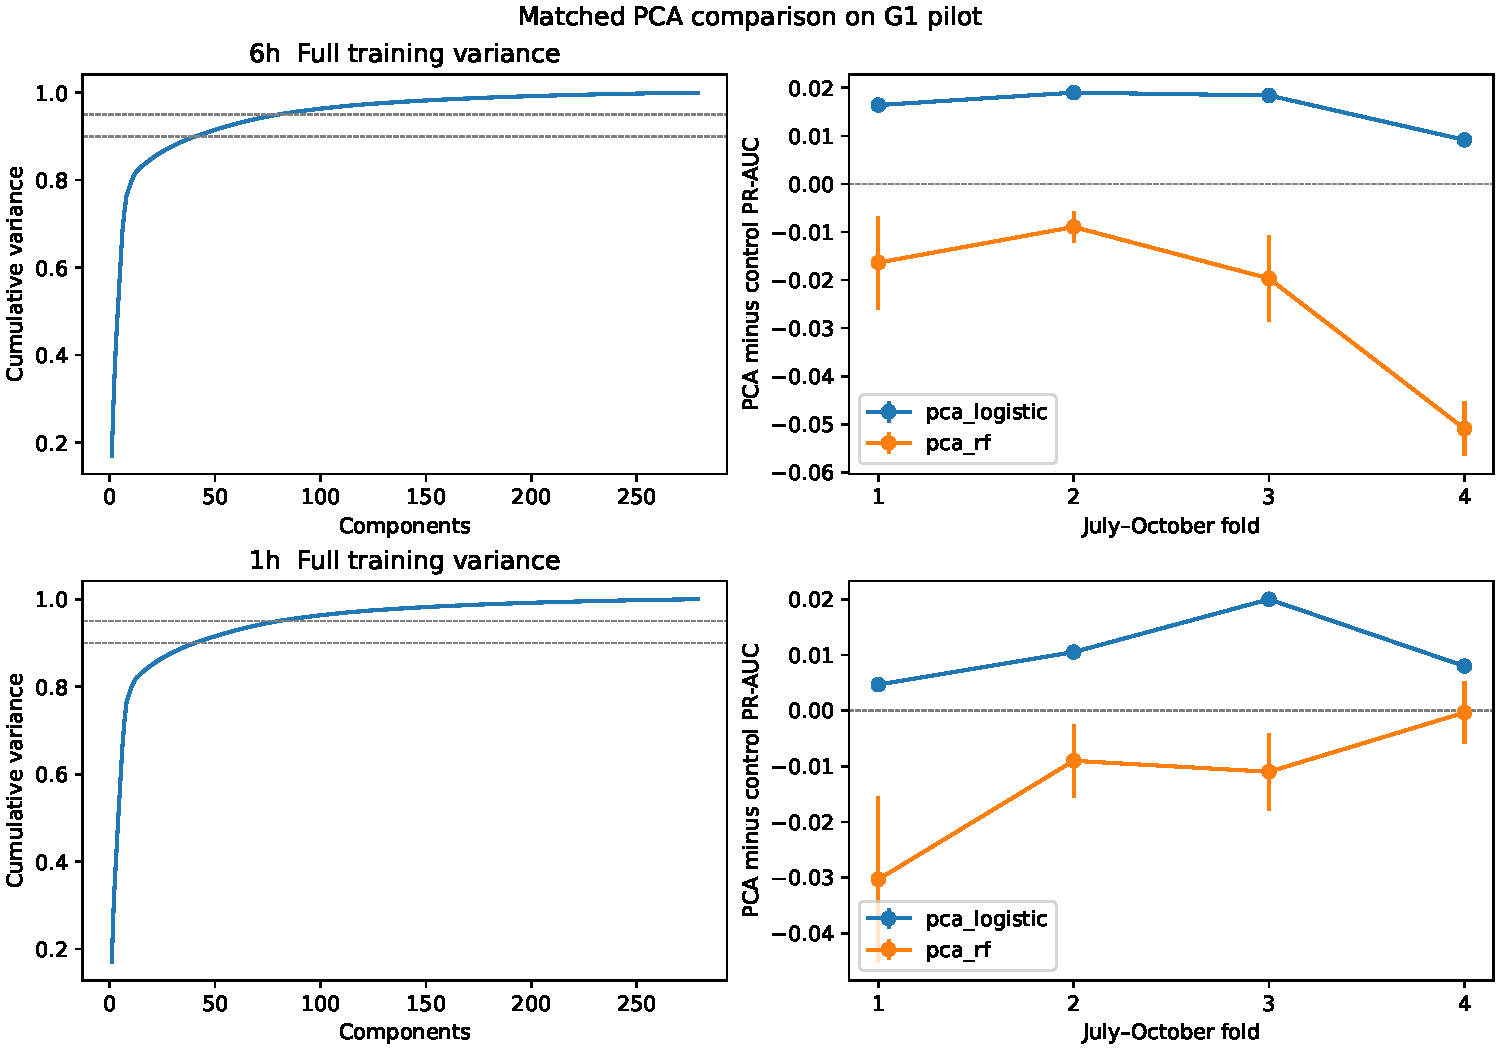
\includegraphics[width=\linewidth]{pca.pdf}
\caption{G1 pilot training-only PCA spectra and paired changes in validation average precision.}
\end{figure}
\begin{figure}[htbp]\centering
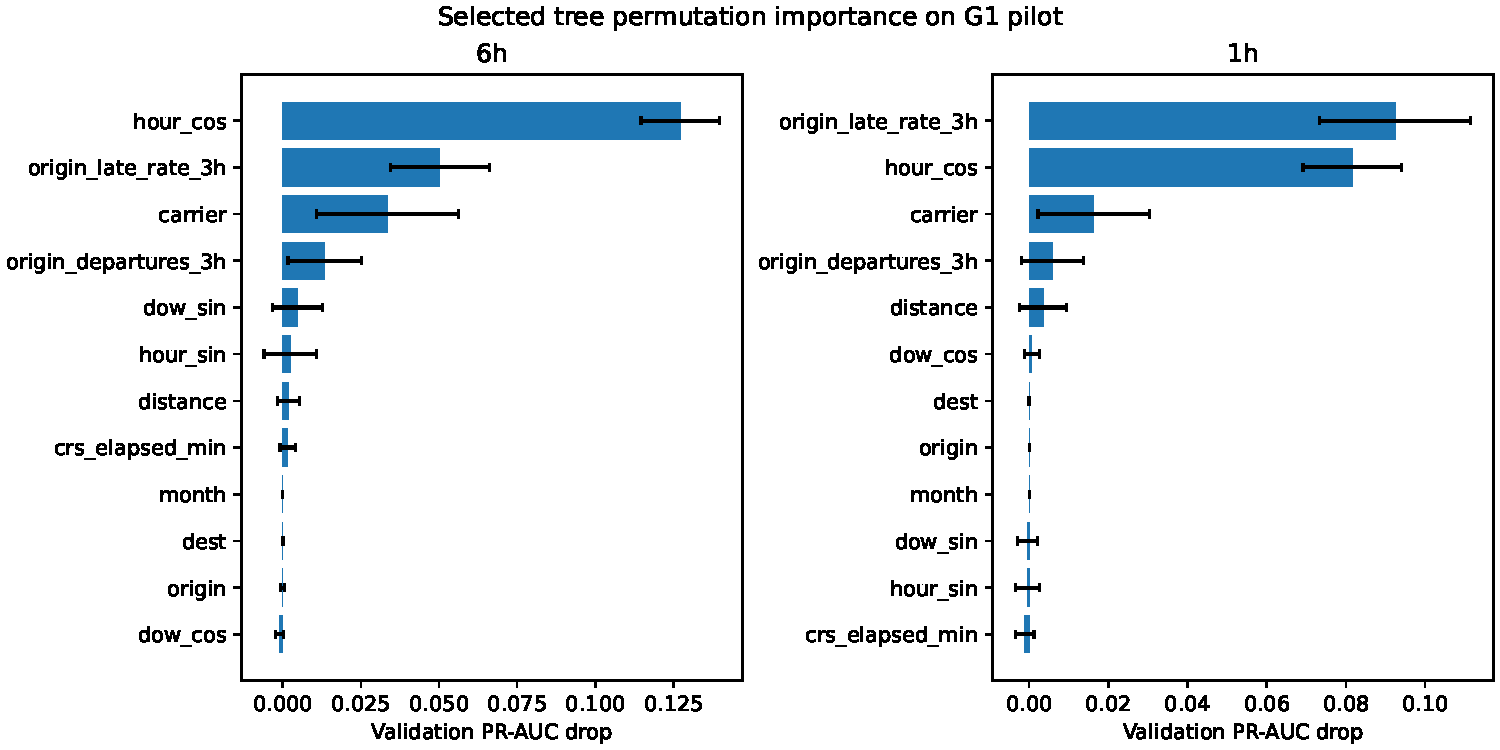
\includegraphics[width=\linewidth]{permutation_importance.pdf}
\caption{Selected G1 tree importance from shuffling original validation predictors.}
\end{figure}
\section{Boosting models}
The development pilot used 20,000 flights at checkpoints six hours and one hour before departure. We compared five boosting families on the same four chronological folds and three training seeds. Each fit chose its iteration count on the trailing fourteen calendar dates inside the training draw, with a one-day gap, before refitting on the outer training draw. We selected the highest mean average precision at each horizon. These estimates describe the development pilot and inform subsequent full-scale tuning.

\begin{center}
\begin{tabular}{lrrrr}
 & \multicolumn{2}{c}{6 hours} & \multicolumn{2}{c}{1 hour} \\
Model & ROC-AUC & PR-AUC & ROC-AUC & PR-AUC \\ \hline
AdaBoost & 0.682 & 0.354 & 0.697 & 0.398 \\
Gradient Boosting & 0.689 & 0.367 & 0.700 & 0.405 \\
XGBoost & 0.697 & 0.383 & 0.700 & 0.415 \\
LightGBM & 0.698 & 0.387 & 0.704 & 0.420 \\
CatBoost & 0.693 & 0.376 & 0.703 & 0.409 \\
\end{tabular}
\end{center}

At 6 hours, LightGBM achieved mean average precision 0.387 (fold--seed standard deviation 0.067). At a 10\% alert budget, precision was 46.0\% and lift was 2.15 times fold prevalence. The largest mean absolute permutation SHAP contributions in the October sample came from the cosine of scheduled UTC departure hour and the origin airport's late-departure rate over the previous three hours.

At 1 hour, LightGBM achieved mean average precision 0.420 (fold--seed standard deviation 0.061). At a 10\% alert budget, precision was 50.3\% and lift was 2.34 times fold prevalence. The largest mean absolute permutation SHAP contributions in the October sample came from the origin airport's late-departure rate over the previous three hours and the cosine of scheduled UTC departure hour.

Native categorical handling changed CatBoost mean average precision by +0.002 at six hours and -0.002 at one hour compared with one-hot input. For LightGBM the corresponding differences were -0.013 and -0.017. Each comparison uses the best tested settings for each encoding.

The operational comparison covers all ten model configurations at 5\%, 10\% and 20\% alert budgets. An illustrative cost assigns one unit to each alert and five units to each missed delay. The SHAP analysis averages 32 random feature orderings over 128 October validation flights per horizon, using training flights as backgrounds. Correlated features limit causal interpretation.
\begin{figure}[htbp]\centering
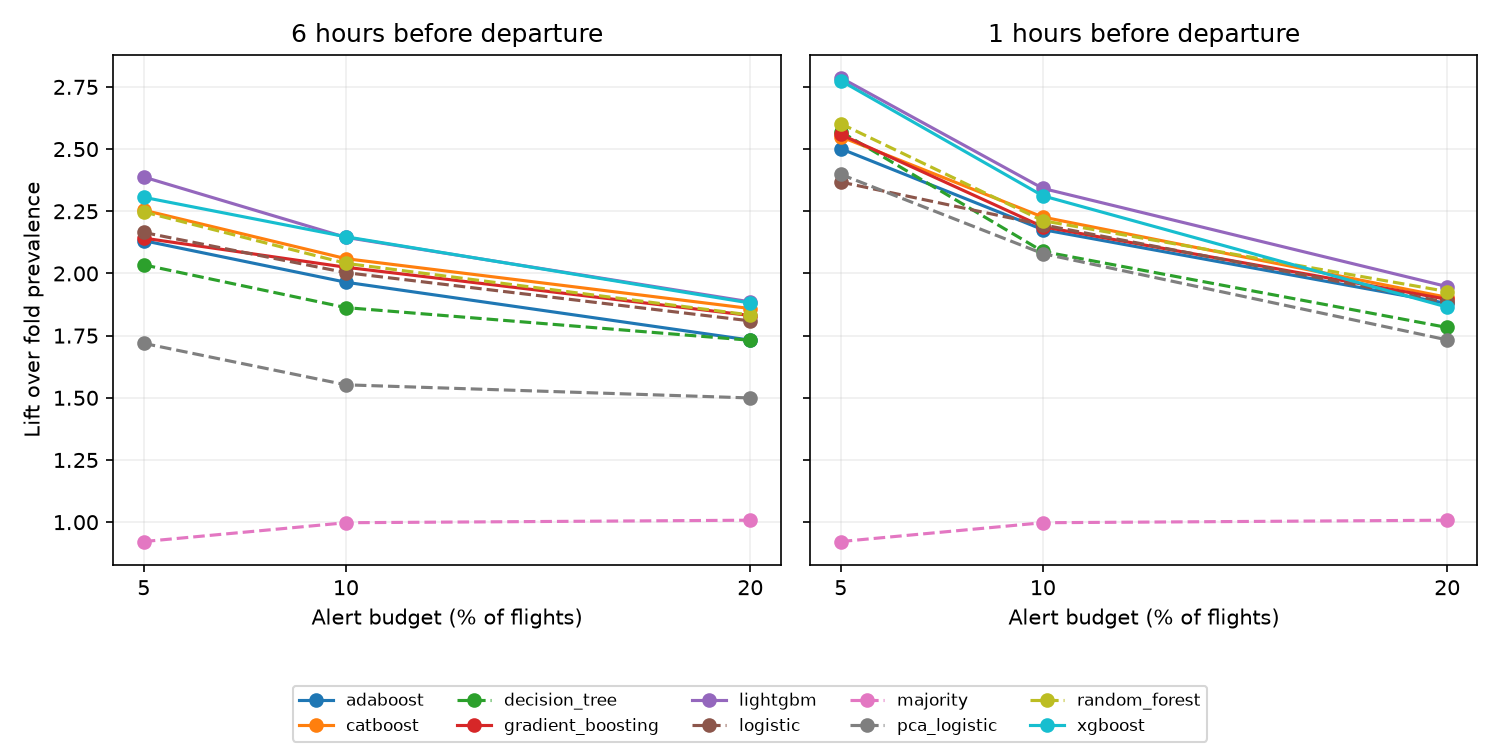
\includegraphics[width=.95\linewidth]{lift.png}
\caption{Validation lift by alert budget at each checkpoint.}
\end{figure}
\begin{figure}[htbp]\centering
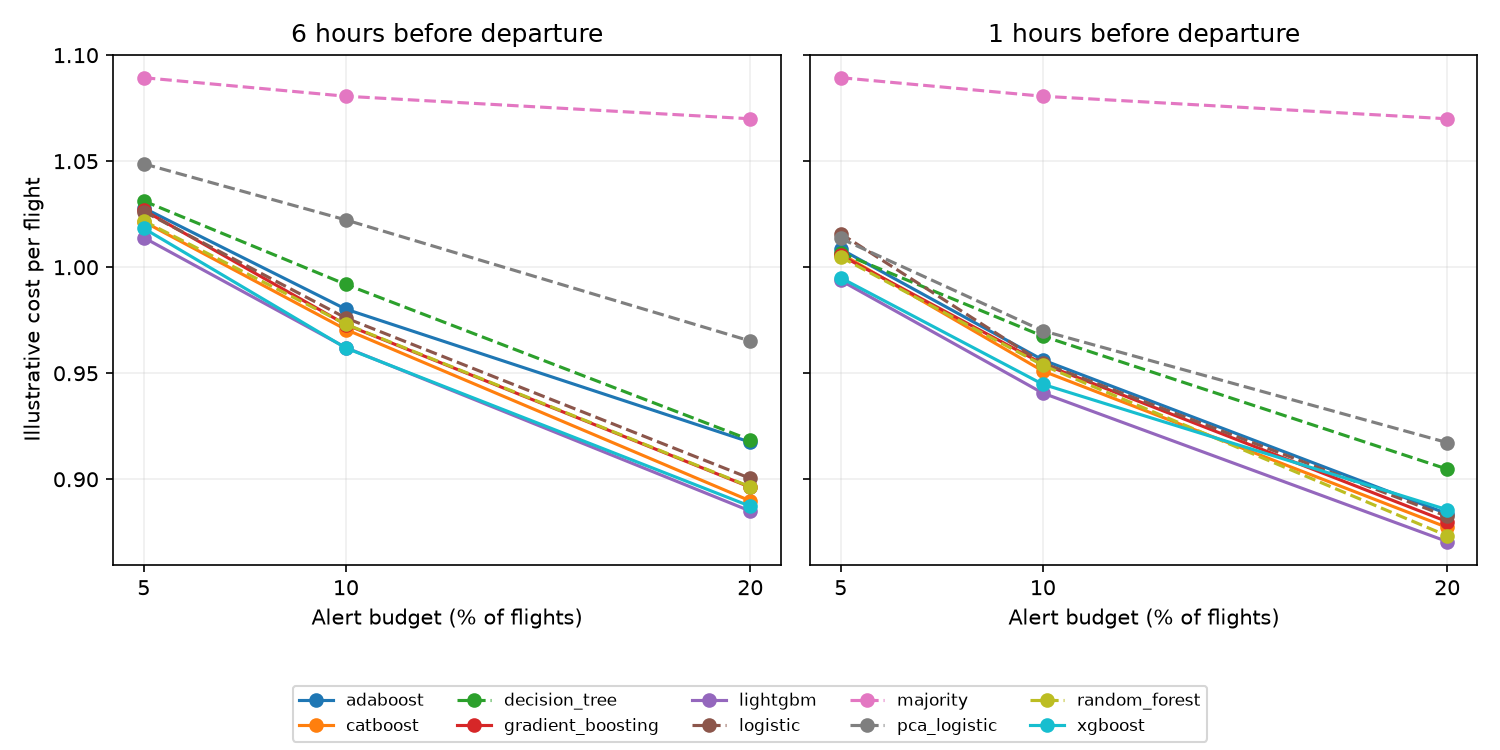
\includegraphics[width=.95\linewidth]{cost.png}
\caption{Illustrative cost per flight as alert capacity changes.}
\end{figure}
\begin{figure}[htbp]\centering
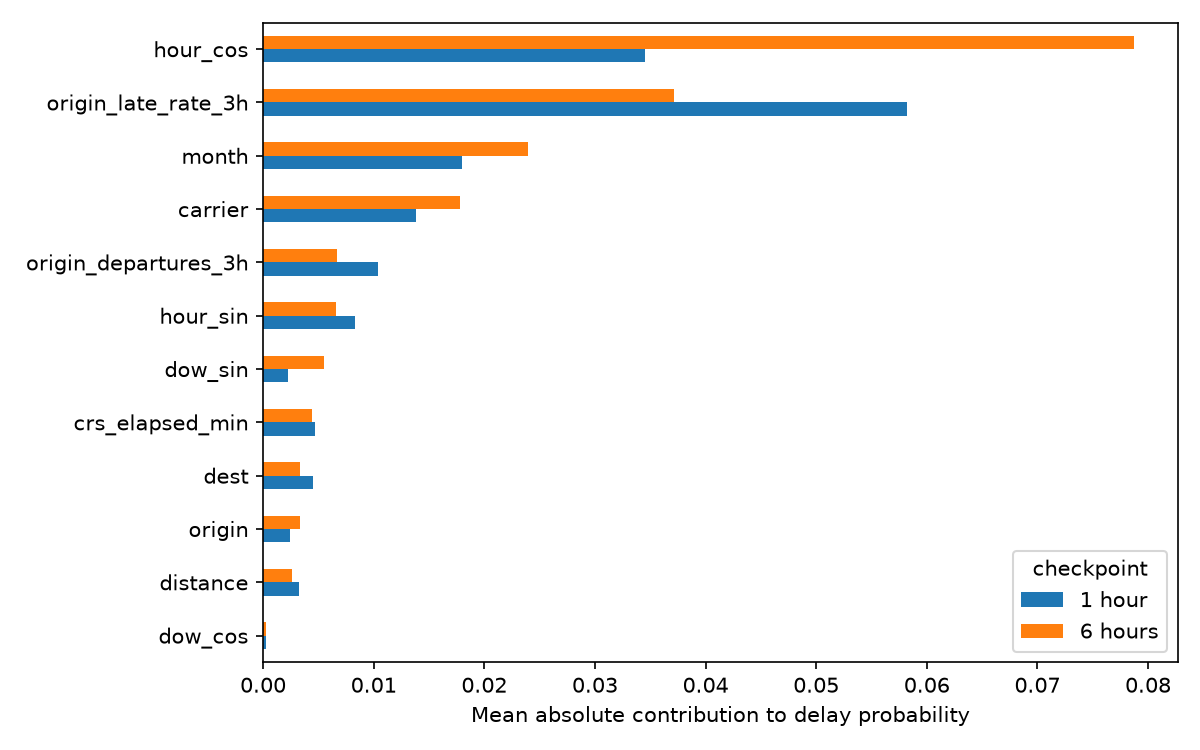
\includegraphics[width=.8\linewidth]{shap.png}
\caption{Mean absolute probability contributions on the October pilot sample.}
\end{figure}
\section{Results}
Owner: P4/P5. Pending reviewed contribution.
\section{Extra analysis}
Owner: Shared, coordinated by P2. Pending reviewed contribution.
\section{Limitations}
Owner: P2. Pending reviewed contribution.
Final test starts 2025-11-02 UTC. Test count and results pending final run. Required results: ROC-AUC and average precision mean and population standard deviation across folds and seeds, for both checkpoints. Include majority baseline, Decision Tree, Random Forest, paired PCA/no-PCA classifier and all five boosting methods.
\end{document}
